% LTeX: language=de-DE
\section{Virtuelle Maschine}

\begin{frame}{Virtuelle Maschine}
	\begin{itemize}
		\item Oft bezeichnet eine \emph{virtuelle Maschine} (VM) ein Softwareprogramm, welches einen echten Computer simuliert
		\item Hierbei werden oft auch Geräte wie das Display, Lautsprecher oder die Festplatte miteinbezogen
		\item In diesem Kontext bezeichnet der Begriff jedoch eine Software, die wie die CPU eines Rechners funktioniert
	\end{itemize}
\end{frame}

\begin{frame}{Wie eine CPU Programme ausführt}
	\begin{itemize}
		\item Die meisten Prozessoren basieren auf der \emph{von Neumann Architektur}~\scite[p.~172]{Ledin2020-yp}
		\item Eine CPU enthält nach von Neumann ein \emph{Rechenwerk}\footnote{Engl: \enquote{arithmetic logic unit} (ALU).}, \emph{Steuerwerk}\footnote{Engl: \enquote{control unit}.}, \emph{Speicherwerk}, \emph{Ein- / Ausgabewerk} und ein Bussystem~\scite[p.~172]{Ledin2020-yp}
		\item Die Programmausführung wird durch den sog. \emph{Befehlszyklus}\footnote{Engl: \enquote{fetch-decode-execute cycle}.} modelliert~\scite[pp.~208-209]{Ledin2020-yp}:
		\item[] \begin{enumerate}
				\item \textbf{Fetch} (Befehl laden): Das Steuerwerk lädt die nächste Anweisung aus dem Speicher
				\item \textbf{Decode} (Befehl dekodieren): Der Befehlscode und die Operanden werden ermittelt
				\item \textbf{Execute} (Befehl ausführen): Die zuständige Einheit im Prozessor wird verwendet, um den Befehl zu verarbeiten.
				      Beispielsweis wird das Rechenwerk für logische und mathemtische Befehle aufgerufen.
			\end{enumerate}
	\end{itemize}
\end{frame}

\begin{frame}{Übertragung der Konzepte auf die rush VM}
	\Lirsting[ranges={16-26}, caption={Struct Definition der VM.}, label={lst:vm_struct}, fancyvrb={fontsize=\footnotesize}, float=H]{deps/rush/crates/rush-interpreter-vm/src/vm.rs}
	\begin{itemize}
		\item \TODO{fix broken caption}
		\item \qVerb{stack}: Speicher für temporäre Werte bei komplexeren Operationen
		\item \qVerb{mem}: Anhaltender Speicher mit einer festen Größe für Variablen
		\item \qVerb{mem_ptr}: Hält den Index der letzten freien Speicherzelle in \qVerb{mem}
		\item \qVerb{call_stack}: Aufrufstapel, welcher den \emph{Befehlsähler} und den \emph{Funktionszähler} für jeden Aufruf speichert
	\end{itemize}
\end{frame}

\begin{frame}{Speicherstruktur der rush VM.}
	\begin{itemize}
		\item Unterscheidung zwischen zwei Arten der Adressierung
		\item \emph{relative Adressierung}: \qVerb{svari *rel[0]}
		\item \emph{absolute Adressierung}: \qVerb{svari *abs[0]}
	\end{itemize}

	\begin{figure}
		\centering
		\begin{NiceTabular}{>{\scriptsize}c}[name=Left]
			\\
			\\
			\\
			num              \\
			\Block[draw]{} 9 \\
		\end{NiceTabular}\hspace{1cm}
		\begin{NiceTabular}
			[
				first-col,
				%code-for-first-col=\ValueMinusOne{iRow},
				first-row,
				hvlines,
				colortbl-like,
				name = Right
			]
			{cc>{\scriptsize}c}
			 & cell                  & rel    & {\normalsize abs} \\
			 & a                     & $-3$   & $mp + rel = 0$    \\
			 & b                     & $-2$   & $mp + (-2) = 1$   \\
			 & c                     & $-1$   & $mp - 1 = 2$      \\
			 & d                     & $0$    & $3$               \\
			 & \cellcolor{gray!30} e & $1$    & $mp + 1 = 4$      \\
			 & \ldots                & \ldots & \ldots            \\
		\end{NiceTabular}

		\begin{tikzpicture}[overlay,remember picture]
			\draw [->] (Left-5.5-|Left-last) to [bend left] (Right-5.5-|Right-1);
			\draw [thick, dashed] (Right-4.5-|Right-5) --  node[anchor=west, xshift=-1cm, align=center] {\scriptsize memory\\ \scriptsize pointer $= 3$} ([xshift=2.5cm]Right-4.5-|Right-4);
		\end{tikzpicture}
		\caption{Speicherstruktur der rush VM.}\label{fig:rush_vm_linmem}
	\end{figure}
\end{frame}

\begin{frame}{Ein Beispielprogramm der rush VM}
	\hspace{0pt} % This is somehow required
	\vfill
	\Lirsting[caption={Beispielprogramm der rush VM.}, fancyvrb={fontsize=\footnotesize}, float=H]{deps/paper/listings/vm_faster_instructions.s}
	\vfill
\end{frame}

\begin{frame}{Struktur der Programme der rush VM}
	\begin{itemize}
		\item Verwendung eines Stacks für Funktionsaufrufe und temporäre Operationen
		\item Unterteilung in Funktionen
		\item Jede Funktion enthält mehrere Anweisungen
		\item Die Funktions- und Variablennamen wurden durch Indizes ersetzt
		\item Im Git Commit \enquote{\rushCommit{}} beinhaltete die VM ca.\ verschiedene 30 Befehlscodes
		\item Jede Anweisung besteht aus einem Befehlscode mit einem optionalen Operanden
		\item Beispiele: \enquote{\LirstInline{asm}{add}} oder \enquote{\LirstInline{asm}{call 2}}
	\end{itemize}
\end{frame}

\begin{frame}{VM: Fazit}
	\begin{itemize}
		\item Ca. 2.7 mal schneller als der tree-walking interpreter
		\item Implementierung des Compilers stellte sich als eher einfach heraus
		\item Die Stack-basierte Architektur erleichterte die Implementierung des Compilers
		\item Gleichzeitige Entwicklung der VM und des Compilers erleichterte einige Vorgänge
		\item Der Compiler profitiert von dem hohen Abstraktionsgrad der VM
	\end{itemize}
\end{frame}

\begin{frame}{VM: Demonstration}
	\Lirsting[float=H, fancyvrb={frame=none, fontsize=\footnotesize}]{listings/pow.rush}
\end{frame}

\begin{frame}{VM: Demonstration}
	\begin{center}
		\href{run:assets/01_rush_presentation_vm.mp4}{
			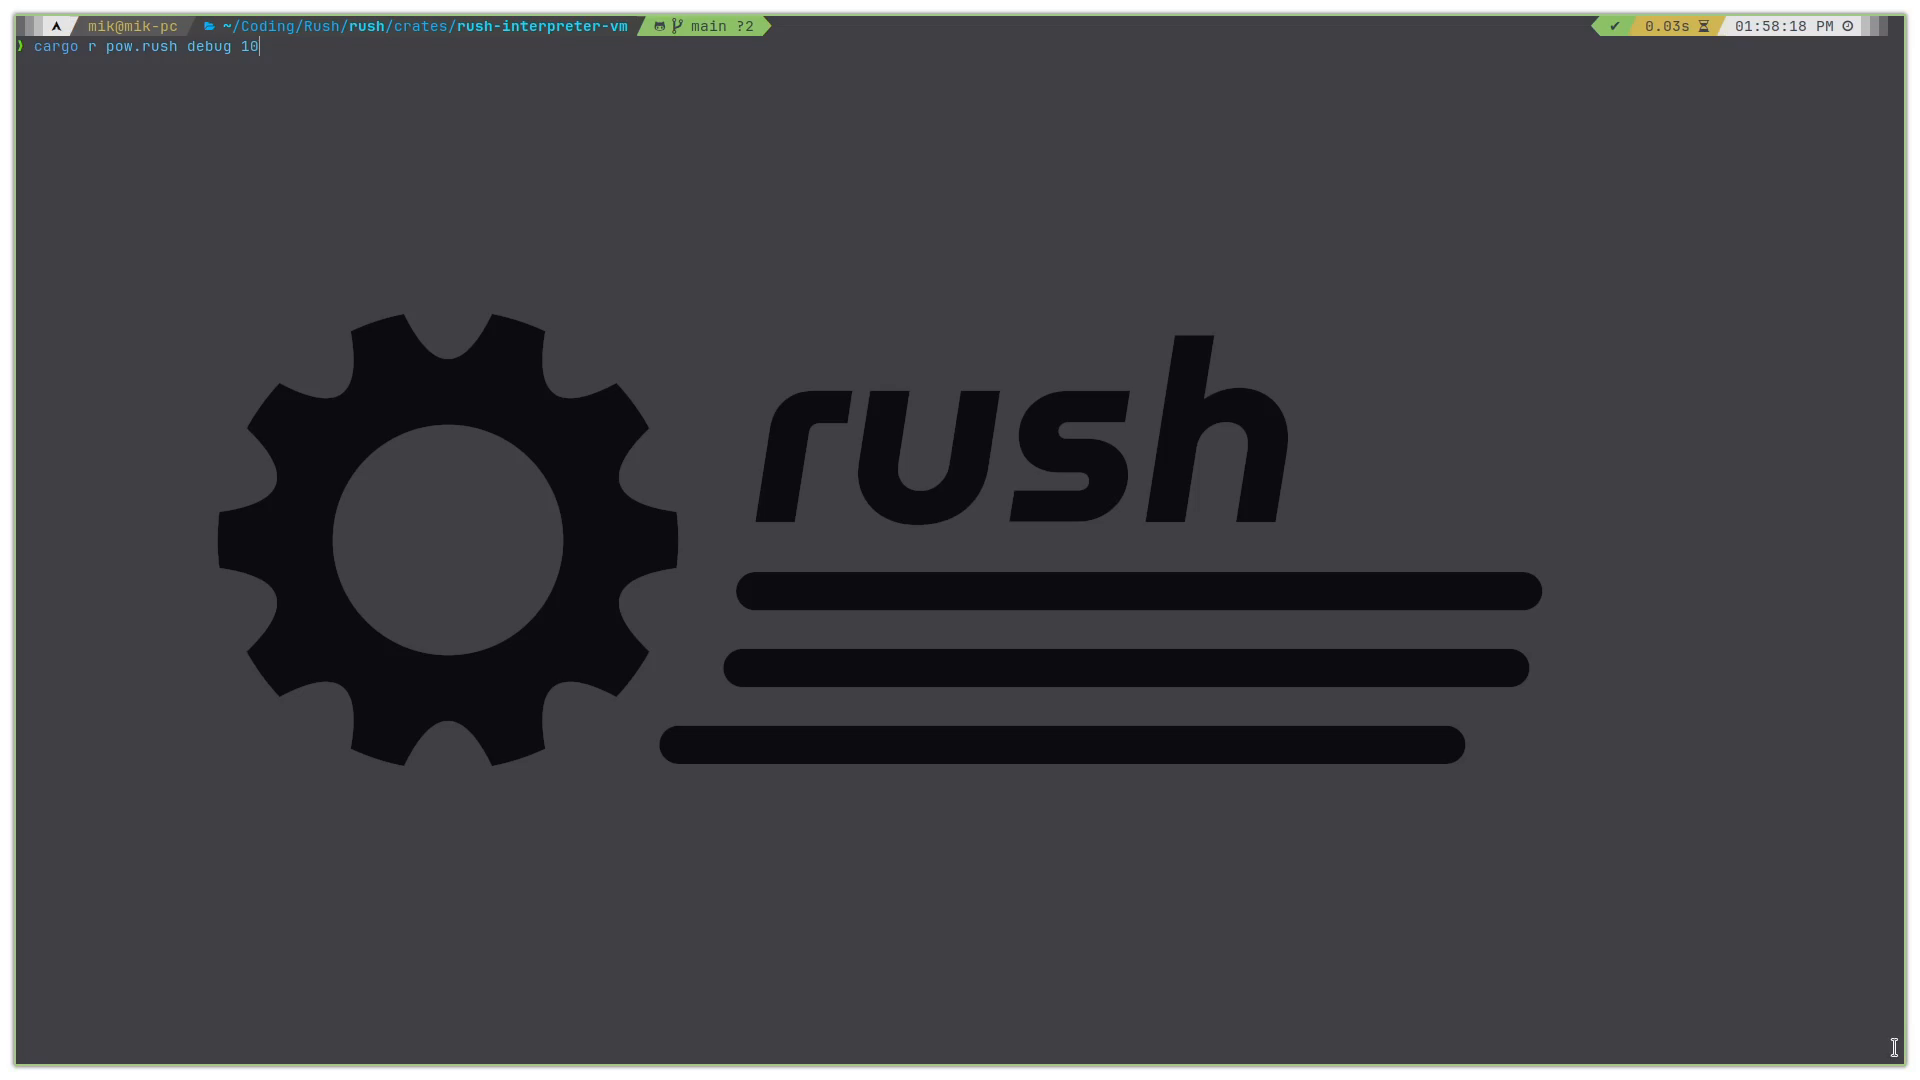
\includegraphics[width=\textwidth]{assets/01_rush_presentation_vm.png}
		}
	\end{center}
\end{frame}
